\documentclass[11pt]{beamer}
\usetheme{Madrid}
\usepackage[utf8]{inputenc}
\usepackage[french]{babel}
\usepackage[T1]{fontenc}
\usepackage{amsmath}
\usepackage{amsfonts}
\usepackage{amssymb}

\def\gint{\displaystyle\int}

\author[Matthieu Brachet]{\underline{M. Brachet}, J.-P. Croisille}
\title[Schémas compacts sur la sphère]{Approximation numérique d'équations aux dérivées partielles sur la sphère par un schéma compact}
\institute[IECL]{Institut Elie Cartan de Lorraine (Metz)} 
\date{28 novembre 2016} 
%\subject{} 
\begin{document}

\begin{frame}
\titlepage
\includegraphics[scale=0.3]{iecl.jpg}
\end{frame}

%% ***********************************************************************
\section*{Introduction}

\begin{frame}{Introduction}
\begin{block}{Objectif}
Discrétisation intrinsèque d'opérateurs sur la sphère.
\end{block}

\begin{equation*}
grad(h) = \nabla h \hspace{1cm} div(\mathbf{u}) = \nabla \cdot \mathbf{u} \hspace{1cm} rot(\mathbf{u}) = \nabla \wedge \mathbf{u}
\end{equation*}

\pause
\begin{block}{Applications}
Résolution d'EDP sur la sphère, notamment en climatologie et en océanographie numérique.
\end{block}

\end{frame}


\begin{frame}

\begin{columns}
\column{0.45\textwidth}
\begin{block}{Equation d'advection :}
\begin{equation}
\left\lbrace
\begin{array}{rcl}
\partial_t h + \mathbf{c} \cdot \nabla h & = & 0 \\
h_{|t=0} & = & h_0 \\
\end{array}
\right.
\end{equation}
\end{block}

\column{0.45\textwidth}
\begin{center}
\includegraphics[scale=0.25]{earth.jpg}
\end{center}

\end{columns}

\pause
\begin{block}{Equation Shallow Water}
\begin{equation}
\left\lbrace
\begin{array}{rcl}
\partial_t h^{\star} + \nabla \cdot \left( h^{\star} \mathbf{u} \right) & = & 0 \\
\partial_t \mathbf{u} + \nabla \left[ \dfrac{1}{2} \mathbf{u}^2 + gh \right] + \left[f + \left( \nabla \wedge \mathbf{u} \right) \cdot \mathbf{k} \right] \mathbf{k} \wedge \mathbf{u} & = & \mathbf{0} \\
\end{array}
\right.
\end{equation}

avec $h^{\star} = h - h_s$ et $h_s$ la topographie.
\end{block}

\end{frame}

%% ***********************************************************************
\begin{frame}
\tableofcontents
\end{frame}

%% ***********************************************************************
\section{Maillage Cubed-Sphere}
\begin{frame}{Maille "Cubed-Sphere" (CS)}

\begin{columns}
\column{0.45\textwidth}
Maillage Latitude-Longitude :

\begin{center}
\includegraphics[scale=0.2]{latlon.png}
\end{center}


\column{0.45\textwidth}
\begin{alertblock}{}
Singularités aux pôles !
\end{alertblock}

\pause
Introduction de la Cubed-Sphere par [R. Sadourny 1972].
\end{columns}

\end{frame}

\begin{frame}

\textbf{Construction via les grands cercles (Panel I) :}

\begin{columns}
\column{0.45\textwidth}

\vspace{0.8cm}
\textbf{Réseau $\xi$ :}

Deux pôles :
\begin{itemize}
\item Nord $(0,0,R)$,
\item Sud $(0,0,-R)$,
\end{itemize}

$\Rightarrow$ Réseau de grands cercles

\includegraphics[scale=0.2]{fig72.jpg}

\pause
\column{0.45\textwidth}

\textbf{Réseau $\eta$ :}

Deux pôles :
\begin{itemize}
\item Est $(0,R,0)$,
\item Ouest $(0,-R,0)$,
\end{itemize}

$\Rightarrow$ Réseau de grands cercles

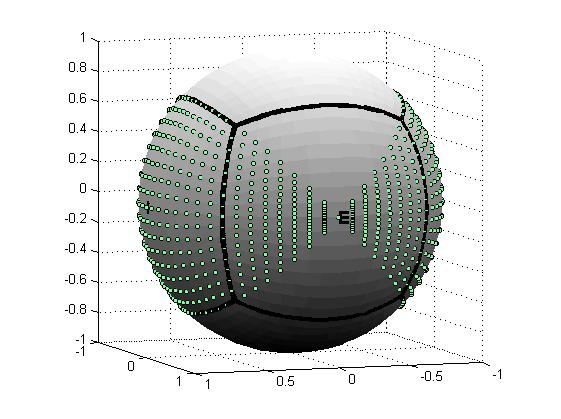
\includegraphics[scale=0.25]{fig22.jpg}

\end{columns}
\end{frame}


\begin{frame}
\begin{columns}
\column{0.45\textwidth}
\tiny
\begin{figure}
\def\svgwidth{0.55 \textwidth}
\vspace{0.5cm}
\input{drawing12.pdf_tex}
\end{figure}
\begin{figure}
\begin{center}
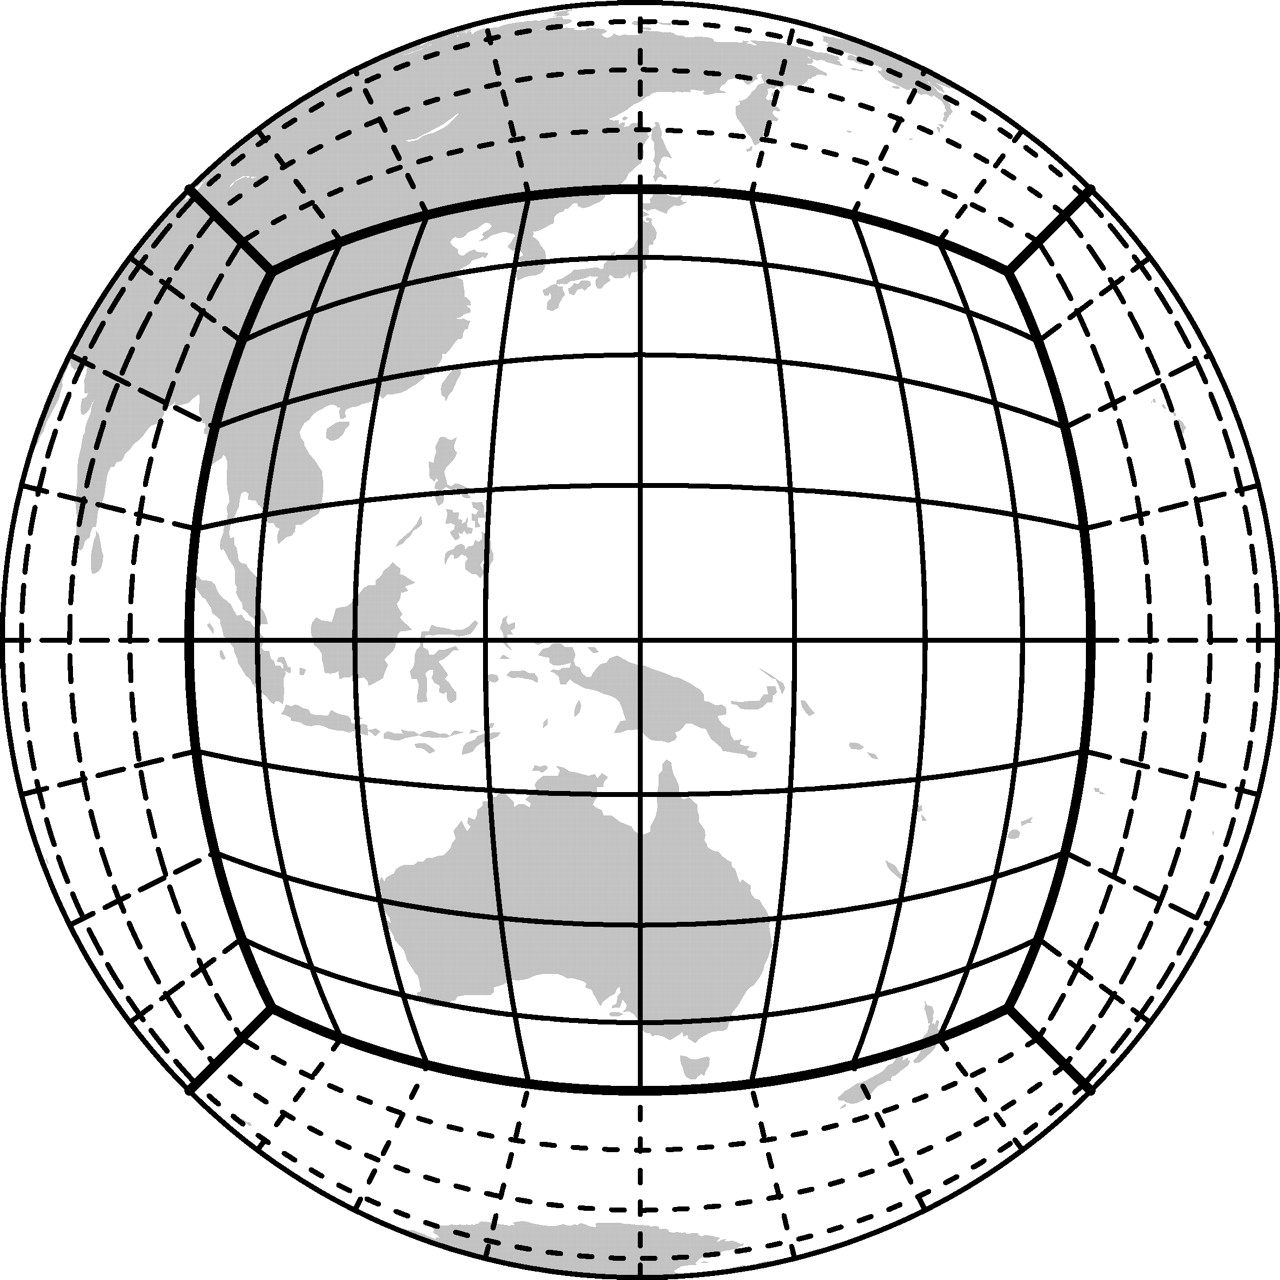
\includegraphics[scale=0.06]{CS_grid.jpg}
\end{center}
\end{figure}

\column{0.45\textwidth}
\begin{itemize}
\item 6 réseaux de cercles géodésiques $C_i^{(1)}$ et $C_j^{(2)}$ , $-N/2 \leq i,j \leq N/2$,
\pause

\item $\mathbf{x}_{i,j}=C_i^{(1)} \cap C_i^{(2)}$
\pause

\item Grille sphérique quasi-cartésienne,
\pause

\item $C_0^{(1)}$ et $C_0^{(2)}$ se coupent à $90^o$,
\pause

\item Grille Cubed-Sphere : 6 panels de $(N+1) \times (N+1)$ points couvrant la sphère.
\end{itemize}
\end{columns}
\end{frame}


\begin{frame}{Métrique sur un panel de la Cubed-Sphere :}
\begin{columns}
\column{0.45\textwidth}
\begin{figure}
\begin{center}
\includegraphics[scale=0.2]{xieta.png}
\end{center}
\caption{1 panel}
\end{figure}

\column{0.45\textwidth}

Coordonnées locales : angles équatoriaux $- \pi/4 \leq \xi, \eta \leq \pi/4$ pour chaque panel :

\begin{itemize}
\item $(\xi_{I}, \eta_{I})$,

\item $(\xi_{II}, \eta_{II})$,

\item $(\xi_{III}, \eta_{III})$,

\item $(\xi_{IV}, \eta_{IV})$,

\item $(\xi_{V}, \eta_{V})$,

\item $(\xi_{VI}, \eta_{VI})$.

\end{itemize}


\end{columns}
\end{frame}


\begin{frame}

Si $\mathbf{x}$ est un point de la sphère de rayon $R$ : $\mathbb{S}_R^2$ du panel I

\begin{itemize}
\item base locale : $(\mathbf{g}_{\xi}, \mathbf{g}_{\eta} ) = ( \partial_{\xi} \mathbf{x}, \partial_{\eta} \mathbf{x} )$,
\pause


\item Introduction d'une métrique $\mathbf{G}$ (Panel I) :

\begin{equation}
\mathbf{G} = \begin{pmatrix}
\mathbf{g}_{\xi} \cdot \mathbf{g}_{\xi} & \mathbf{g}_{\xi} \cdot \mathbf{g}_{\eta} \\ 
\mathbf{g}_{\eta} \cdot \mathbf{g}_{\xi} & \mathbf{g}_{\eta} \cdot \mathbf{g}_{\eta}
\end{pmatrix} =
\dfrac{R^2}{\delta^4} (1+X^2)(1+Y^2)
\begin{pmatrix}
1+X^2 & -XY \\ 
-XY & 1+Y^2 \\
\end{pmatrix}
\end{equation}

avec $X=tan(\xi) = \dfrac{y}{x}$, $Y=tan(\eta) = \dfrac{z}{x}$ et

$\delta = \sqrt{1+X^2+Y^2}$.
\pause

\item Base duale $(\mathbf{g}^{\xi}, \mathbf{g}^{\eta})$ :

\begin{equation}
\left\{
\begin{array}{ccc}
G_{1,1}\mathbf{g}^{\xi} + G_{1,2}\mathbf{g}^{\eta} & = & \mathbf{g}_{\xi} \\ 
G_{2,1}\mathbf{g}^{\xi} + G_{2,2}\mathbf{g}^{\eta} & = & \mathbf{g}_{\eta} \\ 
\end{array} 
\right.
\end{equation}


\end{itemize}
\end{frame}



%% ***********************************************************************
\section{Discrétisation des opérateurs sphériques sur la CS}
\begin{frame}{Discrétisation}

Ecriture d'opérateurs classiques en coordonnées :

\begin{block}{Opérateurs}
Soient $\mathbf{u} : \mathbb{S}_R^2 \longrightarrow \mathbb{T}\mathbb{S}_R^2$ et $h : \mathbb{S}_R^2 \longrightarrow \mathbb{R}$ alors :

\begin{itemize}
\item $grad(h) = \nabla h = \mathbf{g}^{\xi} \dfrac{\partial h}{\partial \xi} + \mathbf{g}^{\eta} \dfrac{\partial h}{\partial \eta}$\\

\item $rot( \mathbf{u} ) =\nabla \wedge \mathbf{u} = \mathbf{g}^{\xi} \wedge \dfrac{\partial \mathbf{u}}{\partial \xi} + \mathbf{g}^{\eta} \wedge \dfrac{\partial \mathbf{u}}{\partial \eta}$\\

\item

\begin{tabular}{rcl}
$div(\mathbf{u})$ & $=$ & $\mathbf{g}^{\xi} \cdot \dfrac{\partial \mathbf{u}}{\partial \xi}+\mathbf{g}^{\eta} \cdot \dfrac{\partial \mathbf{u}}{\partial \eta}$\\
                  & $=$ & $\dfrac{1}{\sqrt{\overline{\mathbf{G}}}} \left[ \dfrac{\partial}{\partial \xi} \left( \sqrt{\overline{\mathbf{G}}} \mathbf{u} \cdot \mathbf{g}^{\xi} \right) + \dfrac{\partial}{\partial \eta} \left( \sqrt{\overline{\mathbf{G}}} \mathbf{u} \cdot \mathbf{g}^{\eta} \right) \right]$
\end{tabular}
\end{itemize}
\end{block}

avec $\overline{\mathbf{G}} = |det(\mathbf{G})|$.
\end{frame}

\begin{frame}{Approximation de $\partial_x u(x_j)$ sur grille cartésienne}
$u_{j+k}$ approximation de $u(x_j + k h)$.
\begin{block}{Approximation d'ordre 2 : $\delta_x u_j$}
\begin{equation*}
\bullet \;\;\; \delta_x u_j = \dfrac{u_{j+1}- u_{j-1}}{2h}
\end{equation*}
\begin{equation*}
\bullet \;\;\; \delta_x u_j = \partial_x u(x_j) + \dfrac{h^2}{6} \partial^{(3)}_x u(x_j) + \mathcal{O}\left( h^4 \right)
\end{equation*}
\end{block}

\pause
Utilisation de schémas compacts [S. K. Lele 1991].

\begin{block}{Approximation d'ordre 4 : $\bar{\delta}_x u_j$}
\begin{equation*}
\bullet \;\;\; \dfrac{1}{6}\bar{\delta}_x u_{j+1}+\dfrac{2}{3}\bar{\delta}_x u_{j} + \dfrac{1}{6}\bar{\delta}_x u_{j-1} = \dfrac{u_{j+1}- u_{j-1}}{2h}
\end{equation*}

\begin{equation*}
\bullet \;\;\; \bar{\delta}_x u_{j} = \partial_x u(x_j) - \dfrac{h^4}{180} \partial^{(5)}_x u (x_j) + \mathcal{O}\left( h^6 \right)
\end{equation*}
\end{block}
\end{frame}

\begin{frame}
En utilisant la périodicité sur les grands cercles :
\begin{equation}
P \delta_{\xi}U_j = Q U_j
\end{equation}

avec $U=(u_{1,j}, ..., u_{4N,j})^T$ et $\delta_{\xi} U=(u_{\xi,1,j}, ..., u_{\xi,4N,j})^T$.

Les matrices :

\begin{equation*}
P=\dfrac{1}{6}\begin{pmatrix}
4 & 1 &   &   1 \\
1 &4 &1&       \\
    & \ddots & \ddots &  \ddots & \\
1 &        &    1 & 4\\
\end{pmatrix} \hspace{1cm} Q=\dfrac{1}{2 \Delta \xi}\begin{pmatrix}
0 & 1 &   &   -1 \\
-1 &0 &1&       \\
    & \ddots & \ddots &  \ddots & \\
1 &        &    -1 & 0\\
\end{pmatrix}
\end{equation*}

\textbf{Remarque :} existence de solveurs rapides basés sur la FFT et la formule de Shermann-Morisson-Woodbury.

\end{frame}

\begin{frame}
\begin{center}
\includegraphics[scale=0.2]{interp.png}
\end{center}

Utilisation de la spline cubique pour compléter les grands cercles.

\end{frame}

\begin{frame}{Convergence}

\begin{block}{Proposition :}
Les versions discrètes de la divergence (formule 1), du gradient et du rotationnel sont d'ordre 3 :

\begin{itemize}
\item gradient :
$$
\| \nabla h - \nabla_{\text{disc}} h  \| = \mathcal{O}\left( \Delta \xi^3, \Delta \eta^3 \right)
$$
\item divergence :
$$
\| \nabla \cdot \mathbf{u} - \nabla_{\text{disc}} \cdot \mathbf{u} \| = \mathcal{O}\left( \Delta \xi^3, \Delta \eta^3 \right)
$$
\item rotationnel :
$$
\| \nabla \wedge \mathbf{u} - \nabla_{\text{disc}} \wedge \mathbf{u}  \| = \mathcal{O}\left( \Delta \xi^3, \Delta \eta^3 \right)
$$
\end{itemize}
\end{block}

\textbf{Remarque :} Dans la pratique, on observe des convergence à l'ordre 4.
\end{frame}




%% ***********************************************************************
\section{Equation d'advection sphérique}
\begin{frame}{Equation d'advection sphérique}

\begin{itemize}
\item $(\lambda, \theta)$ : système de coordonnées classiques,
\item $(\lambda', \theta')$ : système de coordonnées tournées d'un angle $\alpha$.
\end{itemize}

\begin{columns}
\column{0.45\textwidth}
\begin{figure}
\def\svgwidth{0.6 \textwidth}
\vspace{0.5cm}
\input{drawing34.pdf_tex}
\end{figure}

\column{0.45\textwidth}
\begin{block}{Equation d'advection sphérique}
\begin{equation}
\left\lbrace
\begin{array}{rcl}
\partial_t h+ \mathbf{c}(\mathbf{x},t)\cdot \nabla h &=& 0 \\
h(\mathbf{x},0) &=& h_0(\mathbf{x}) 
\end{array}
\right.
\label{eq:advection}
\end{equation}

avec $\mathbf{x} \in \mathbb{S}_R^2$ et $t>0$
\end{block}


\end{columns}


\end{frame}

\begin{frame}
\begin{block}{Proposition : Déplacement sans déformation}
Si $\mathbf{c}(\mathbf{x},t)=R \omega cos ( \theta') \mathbf{e}_{\lambda'}$ alors la solution de \eqref{eq:advection} est :
$$h(\mathbf{x},t)=h_0(P_{\alpha}R_{-t}P_{\alpha}^{-1} \mathbf{x})$$
\end{block}

avec :

\begin{itemize}
\item $R_{-t}$ la rotation autour de $(Oz')$ d'angle $-u_0 cos( \theta' ) t$,

\item $P_{\alpha}$ la rotation autour de $(Ox)$ d'angle $\alpha$.
\end{itemize}

\pause
\textbf{Test 1 de [Williamson 1992]} Bump en rotation solide :

Cas particulier du résultat ci-dessus avec $h_0$ un Bump $\mathcal{C}^1$.

\end{frame}


\begin{frame}{Schéma globale}

\begin{block}{Discrétisation RK4 en temps :}

\begin{enumerate}
\item $K_1 = - \mathbf{c} \cdot \nabla_{\text{disc}} h^n$,

\item $K_2 = - \mathbf{c} \cdot \nabla_{\text{disc}} \left(h^n + \dfrac{\Delta t}{2} K_1\right)$,

\item $K_3 = - \mathbf{c} \cdot \nabla_{\text{disc}} \left(h^n + \dfrac{\Delta t}{2} K_2\right)$,

\item $K_4 = - \mathbf{c} \cdot \nabla_{\text{disc}} \left(h^n + \Delta t K_4\right)$,

\item \textbf{Assemblage :} $h^{n+1} = h^n + \dfrac{\Delta t}{6} \left( K_1 + 2 K_2 + 2 K_3 + K_4  \right)$
\end{enumerate}

\end{block}
\end{frame}

\begin{frame}

\begin{alertblock}{}
Apparition d'ondes parasites !
\end{alertblock}

\begin{columns}
\column{0.45\textwidth}
Mesure de l'erreur relative :

$$e_p^n = \dfrac{\| h(t^n) - h^n \|_p}{\|h(t^n)\|_p}$$

avec $p \in \lbrace 1, 2, \infty \rbrace$.

\column{0.45\textwidth}
\begin{center}
\begin{figure}
\href{run:ref_7363895058_test_0.avi}{\includegraphics[scale=0.25]{ref_7366106674_normerreur_test_0.png}} 
\caption{$N=40$, $CFL=0.9$, $\alpha = \pi /4$}
\end{figure}
\end{center}
\end{columns}

\pause
\begin{block}{}
Ajout d'un filtrage nécessaire.
\end{block}
\end{frame}

\begin{frame}
\begin{enumerate}
\item $K_1 = - \mathbf{c} \cdot \nabla_{\text{disc}} h^n$,

\item $K_2 = - \mathbf{c} \cdot \nabla_{\text{disc}} \left(h^n + \dfrac{\Delta t}{2} K_1\right)$,

\item $K_3 = - \mathbf{c} \cdot \nabla_{\text{disc}} \left(h^n + \dfrac{\Delta t}{2} K_2\right)$,

\item $K_4 = - \mathbf{c} \cdot \nabla_{\text{disc}} \left(h^n + \Delta t K_4\right)$,

\item \textbf{Assemblage :} $\widehat{h}^{n+1} = h^n + \dfrac{\Delta t}{6} \left( K_1 + 2 K_2 + 2 K_3 + K_4  \right)$

\item \textbf{Filtrage :} $h^{n+1} = F(\widehat{h}^{n+1}) $.
\end{enumerate}


\begin{block}{Filtrage Passe-Bas}
\begin{equation}
F_{10}(u)_{i} = \sum_k f_k u_{i+k}
\end{equation}

avec $(f_0, f_1, f_2, f_3, f_4) = \dfrac{1}{1024}(772, 210, -120, 45, -10, 1)$ est un filtre d'ordre 10.

\end{block}
\end{frame}

\begin{frame}
\begin{columns}
\column{0.45\textwidth}

\begin{block}{Ordre du filtrage}
Le filtrage d'ordre élevé pour éviter la perte de qualité.
\end{block}

\column{0.45\textwidth}
\begin{center}
\includegraphics[scale=0.3]{07-Oct-2016ref_7366105937_coupefaceI_equateur_test_0.png}
\end{center}


\end{columns}
\end{frame}

\begin{frame}

\textbf{Schéma numérique :} RK4 + Filtrage d'ordre 10 + Compact 4

\begin{figure}
\begin{center}
\includegraphics[scale=0.3]{ref_7366098300_normerreur_test_0.png}
\end{center}
\caption{Test 1 de [Williamson,1992] }
\end{figure}

\end{frame}

\begin{frame}{Equation de convection avec vitesse dépendant du temps}

\begin{block}{}
\begin{equation}
\left \{
\begin{array}{l}
\dfrac{\partial h}{\partial t} + \mathbf{a}(t,\mathbf{x}) \cdot \nabla_T h = 0\\[6pt]
h(0,\mathbf{x}) = h_0(\mathbf{x})\\
\end{array}
\right.
\label{eq:advection}
\end{equation}
\end{block}

\begin{block}{vitesse de type vortex indépendant du temps}
$\mathbf{a}_r(\mathbf{x}) = \omega_r (\theta') cos ( \theta') \mathbf{e}_{\lambda'}$ vitesse variable du vortex.
\end{block}


\begin{block}{Vitesse globale :
Combinaison de la rotation solide et de la vitesse de type vortex}

$$\mathbf{a}(t, \mathbf{x}) = \underbrace{\mathbf{a}_s ( \mathbf{x} )}_{\text{rotation solide}} + \underbrace{\mathbf{a}_r (t, \mathbf{x})}_{\text{vitesse de type vortex}}$$




\begin{flushright}
[Nair, Jablonowski, 2008]
\end{flushright}
\end{block}

\end{frame}



\begin{frame}
\begin{block}{Solution analytique}
Solution analytique de \eqref{eq:advection} donnée dans $( \lambda', \theta')$, le système de coordonnées associé à l'axe tourné d'un angle $\alpha$, par :

$$h(t, \lambda', \theta') = 1 -tanh \left[ \frac{\rho}{\gamma} sin( \lambda' - \omega_r t ) \right]$$

$\rho$ et $\omega_r$ dépendant de $\theta'$.
\end{block}

\pause
\begin{columns}
\column{0.45\textwidth}
\begin{figure}
\href{run:ref_7363145849_test_2.avi}{\includegraphics[scale=0.25]{14-Oct-2015_normerreur_test_2.png}} 
\caption{maillage $6 \times 40 \times 40$}
\end{figure}

\column{0.45\textwidth}
\begin{figure}
\includegraphics[scale=0.25]{ref_7366148261_coupefaceI_equateur_test_1.png}
\caption{Sous résolution (t=12jours)}
\end{figure}
\end{columns}

\end{frame}


\begin{frame}{Table de convergence pour le test du vortex en déplacement}
\begin{table}
\begin{tabular}{c||cc|cc|cc}
$N$ & $max_n |e_1^n|$ & ordre  & $max_n |e_2^n|$ & ordre  & $max_n |e_{\infty}^n|$ & ordre \\
\hline
\hline
$40$ & $2.7609 (-3)$ & -  & $9.7386 (-3)$ & - & $5.4808 (-2)$  & - \\
\hline 
$50$ & $1.2760 (-3)$ & $3.5364$ & $5.0160 (-3)$ & $3.0399$ & $3.2035 (-2)$ & $2.4605$ \\
\hline
$60$ & $6.2957 (-4)$ & $3.9456$ & $2.6157 (-3)$ & $3.6365$ & $1.8218 (-2)$ & $3.1523$ \\
\hline
$80$ & $1.9603 (-4) $ & $4.1145$ & $8.3722 (-4)$ & $4.0173$ & $6.0931 (-3)$ & $3.8623$ \\
\hline
$100$ & $8.0399 (-5)$ & $4.0389$ & $3.4524 (-4)$ & $4.0143$ & $2.6514 (-3)$ & $3.7706$\\
\hline
$150$ & $1.5656 (-5)$ & $4.0684$ & $6.9199 (-5)$ & $3.9966$ & $5.8082 (-4)$ & $3.7756$
\end{tabular}
\caption{Table de convergence pour le test du vortex en déplacement, $CFL = 0.7$ ; $\alpha = \pi /4$.}\end{table}

\end{frame}



%% ***********************************************************************
\section{Equation Shallow Water}
\begin{frame}{Equation Shallow Water sphérique}
Modèle issu des équations de Navier-Stokes en considèrant :
\begin{itemize}
\item faible épaisseur du fluide comparé à sa largeur,
\item faible viscosité du fluide.
\end{itemize}

\pause
\begin{block}{Equation Shallow Water (Eq. de Saint-Venant)}
\begin{equation}
\left\lbrace
\begin{array}{rcl}
\partial_t h^{\star} + \nabla \cdot \left( h^{\star} \mathbf{u} \right) & = & 0 \\
\partial_t \mathbf{u} + \nabla \left[ \dfrac{1}{2} \mathbf{u}^2 + gh \right] + \left[f + \left( \nabla \wedge \mathbf{u} \right) \cdot \mathbf{k} \right] \mathbf{k} \wedge \mathbf{u} & = & \mathbf{0} \\
\end{array}
\right.
\end{equation}

avec $h^{\star} = h - h_s$ et $h_s$ la topographie.
\end{block}

\begin{itemize}
\item $g$ : force de gravité,
\item $f$ paramètre de la force de Coriolis, $f=2 \omega sin( \theta )$,
\item $\mathbf{k}$ normale extérieure.
\end{itemize}

\end{frame}


\begin{frame}{Relations de Conservation}

\begin{block}{Proposition :}
Les relations de conservation suivantes sont satisfaites :
\begin{itemize}
\item Conservation de la masse :
$$\gint_{\mathbb{S}_R^2} h = Cste$$

\item Conservation de l'énergie :
$$\gint_{\mathbb{S}_R^2} gh^2+\dfrac{1}{2}h \mathbf{u}^2 = Cste$$

\item Conservation de l'enstrophie potentielle :
$$\gint_{\mathbb{S}_R^2} \dfrac{1}{2} \dfrac{\left( (\nabla \wedge \mathbf{u}) \cdot \mathbf{k} + f \right)}{\left( h - h_s\right)} = Cste$$
\end{itemize}
\end{block}

\end{frame}


\begin{frame}

\begin{block}{}
Equation hyperbolique non linéaire
\end{block}

\pause
\begin{itemize}
\item 
Filtrage d'ordre $\geq 6$ : insuffisant : apparition d'ondes parasites aux coins de la CS,

\item Filtrage d'ordre $\leq 6$ : Trop dissipatif.
\end{itemize}

$\Rightarrow$ Construction d'un filtrage adaptatif : filtrage local qui supprime les oscillations.

\end{frame}


\begin{frame}{Filtrage adaptatif}

\begin{enumerate}
\item \textbf{Isoler les fautes fréquences :}
$$u_{hf} = F_{ph} (u) = u - F_{10} (u)$$\\
\item \textbf{Capter les oscillations :}
$$r_i = \dfrac{1}{2}\left[ \left( u_{hf,i+1} - u_{hf,i} \right)^2 + \left( u_{hf,i-1} - u_{hf,i}  \right)^2 \right]$$\\
\item \textbf{Détecteur :} Construction de $\sigma$ tel que
$$\sigma = \psi ( r ) \simeq \left\lbrace
\begin{array}{c}
 1 \text{ lorsque r est grand}\\
 0 \text{ lorsque r est petit}
\end{array}
\right.$$
\item \textbf{Filtrage :}
$$F_a(u_{i}) = \sigma_i F_{4}(u_i) + (1-\sigma_i) u_i$$

\end{enumerate}
\end{frame}

\begin{frame}
\textbf{Comparaison en fréquentiel :}
\begin{figure}
\begin{center}
\includegraphics[scale=0.2]{freqftr.jpg}
\end{center}
\caption{Analyse fréquentielle - Filtrage}
\end{figure}
\end{frame}


\begin{frame}{Test 2 de [Williamson, 1992] : solution stationnaire}

\textbf{Topographie :} absence de reliefs,

\textbf{Solution stationnaire :}
\begin{equation}
h = h_0 - \left( R \omega u_0 + \dfrac{u_0^2}{2} \right) \left( - cos \lambda cos \theta sin \alpha + sin \theta sin \alpha \right)^2
\end{equation}

et $\mathbf{u}=u \mathbf{e}_{\lambda}+ v \mathbf{e}_{\theta}$ :

\begin{equation}
\left\lbrace
\begin{array}{rcl}
u & = & u_0 \left( cos \theta cos \alpha + cos \lambda sin \theta sin \alpha  \right)\\
v & = & - u_0 sin \lambda sin \alpha \\
\end{array}
\right.
\end{equation}

\textbf{Coriolis :}
\begin{equation}
f=2 \omega \left( - cos \lambda cos \theta sin \alpha + sin \theta cos \alpha \right)
\end{equation}
\end{frame}

\begin{frame}
Avec $\alpha = \pi / 4$ :

\begin{center}
\includegraphics[scale=0.35]{ref_7366583958_snapshot_intermediaire1.png}
\end{center}
\end{frame}


\begin{frame}
Avec $\alpha = \pi / 4$ :

\begin{columns}
\column{0.45\textwidth}
\begin{figure}
\includegraphics[scale=0.25]{ref_7366583958_erreur.png}
\caption{Erreur relative}
\end{figure}

\column{0.45\textwidth}
\begin{figure}
\includegraphics[scale=0.25]{ref_7366583958_conservation.png}
\caption{Relations de conservation}
\end{figure}


\end{columns}
\end{frame}
























\begin{frame}{Test 5 de [Williamson, 1992] : montagne isolée}

\begin{equation}
\left\lbrace
\begin{array}{rcl}
\partial_t h^{\star} + \nabla \cdot \left( h^{\star} \mathbf{u} \right) & = & 0 \\
\partial_t \mathbf{u} + \nabla \left[ \dfrac{1}{2} \mathbf{u}^2 + gh \right] + \left[f + \left( \nabla \wedge \mathbf{u} \right) \cdot \mathbf{k} \right] \mathbf{k} \wedge \mathbf{u} & = & \mathbf{0} \\
\end{array}
\right.
\end{equation}

\textbf{Topographie :} sphère 'lisse' avec une montagne conique donnée par :

\begin{equation}
h_s = h_{s_0} \left( 1 - \dfrac{r}{R_m} \right)
\end{equation}

avec $r^2=min(R_m^2, (\lambda-\lambda_c)^2 + (\theta-\theta_c)^2)$.

$(\lambda_c, \theta_c)$ : position de la montagne,
$R_m = \pi / 9$ et $h_{s_0}=2000$ mètres.


\end{frame}

\begin{frame}

\textbf{Condition initiale :} zonale autour de l'équateur (état stationnaire en l'absence de reliefs).

$$h_0(\lambda, \theta)=\eta_0 + \left( R \omega u_0 +\dfrac{u_0^2}{2} \right) sin^2 \theta$$

le champ de vitesse $\mathbf{u} = u \mathbf{e}_{\lambda}+v \mathbf{e}_{\theta}$
$$\left\lbrace
\begin{array}{rcl}
u&=&u_0 cos \theta \\
v&=&0
\end{array}
\right.$$

et $f=2 \omega cos \theta$.

\pause
\vspace{0.8cm}
\begin{itemize}
\item Pas de solution analytique connue,

\item Observation quantitative de la solution à $t=5$, $10$ et $15$ jours,

\item Relations de conservation.
\end{itemize}
\end{frame}


\begin{frame}{Résultats numériques}

\begin{columns}
\column{0.45\textwidth}

\href{run:ref_7366568562.avi}{\includegraphics[scale=0.2]{relief.jpg}}

\column{0.45\textwidth}
\includegraphics[scale=0.25]{ref_7366568562_conservation.png}

\end{columns}
\end{frame}





% ************************************************************************

\section*{Conclusion et perspectives}
\begin{frame}{Conclusion et perspectives}

\begin{block}{}
Méthode basée sur un différences finies centré pour la résolution d'EDP hyperboliques.
\end{block}

\begin{block}{}
\begin{itemize}
\item Etude des opérateurs comme algorithmes de points fixes,

\item Laplacien,

\item Méthodes implicites en temps.
\end{itemize}
\end{block}


\end{frame}

% ************************************************************************
\begin{frame}
\frametitle{Bibliographie}

\begin{thebibliography}{9}
        

\scriptsize{

\bibitem{Lele}
         Sanjiva K. Lele
         \emph{: Compact Finite Difference Schemes with spectral-like resolution}.
         1991.
         
\bibitem{Redonnet}
         Stéphane Redonnet
         \emph{: Simulation de la propagation acoustique en présence d'écoulements quelconques et de structures solides par résolution numérique des équations d'Euler}.
         Thèse, 2001.

\bibitem{Croisille}
         J.-P. Croisille
         \emph{: Hermitian compact interpolation on the cubed-sphere grid}.
         2013.

\bibitem{Nair Jablonowski}
         Ramachandran D. Nair et Christiane Jablonowski
         \emph{: Moving Vortices on the Sphere : A test case for Horizontal Advection Problems}.
         1991.

         
\bibitem{Williamson}
         David L. Williamson, John B. Drake, James J. Hack, Rüdiger Jakob et Paul N.Swarztrauber
         \emph{: A strandard test set for Numerical Approximations to the Shallow Water Equations in Spherical Geometry}.
         1994.
    
    }     
         
         
         
\end{thebibliography}
\end{frame}

\begin{frame}
\begin{center}
Merci de votre attention :)
\end{center}
\end{frame}

\end{document}